% SEE GITHUB REPO AT https://github.com/gboeing/gis-bok-notebooks

\RequirePackage[l2tabu,orthodox]{nag}
\documentclass[11pt,letterpaper]{article}
\usepackage[T1]{fontenc}
\usepackage[utf8]{inputenc}
\usepackage{crimson}
\usepackage{helvet}
\usepackage[strict,autostyle]{csquotes}
\usepackage[USenglish]{babel}
\usepackage{microtype}
\usepackage{authblk}
\usepackage{booktabs}
\usepackage{caption}
\usepackage{endnotes}
\usepackage{geometry}
\usepackage{graphicx}
\usepackage{hyperref}
\usepackage{natbib}
\usepackage{rotating}
\usepackage{setspace}
\usepackage{titlesec}
\usepackage{url}
\usepackage{color, soul}

% location of figure files, via graphicx package
\graphicspath{{./figures/}}

% configure the page layout, via geometry package
\geometry{
	paper=letterpaper,
	top=4cm,
	bottom=4cm,
	left=4cm,
	right=4cm}
\setstretch{1.02}
\clubpenalty=10000
\widowpenalty=10000

% set section/subsection headings as the sans serif font
\titleformat{\section}{\normalfont\sffamily\large\bfseries}{\thesection.}{0.3em}{}
\titleformat{\subsection}{\normalfont\sffamily\small\bfseries}{\thesubsection.}{0.3em}{}

% make figure/table captions sans-serif small font
\captionsetup{font={footnotesize,sf},labelfont=bf,labelsep=period}

% configure pdf metadata and link handling
\hypersetup{
	pdfauthor={Geoff Boeing and Daniel Arribas-Bel},
	pdftitle={GIS and Computational Notebooks},
	pdfsubject={GIS and Computational Notebooks},
	pdfkeywords={GIS,},
	pdffitwindow=true,
	breaklinks=true,
	colorlinks=false,
	pdfborder={0 0 0}}

\title{GIS and Computational Notebooks}
\author{Geoff Boeing and Dani Arribas-Bel}
\date{2020}

\begin{document}

\maketitle

\begin{abstract}
This chapter introduces computational notebooks in the context of GIS. We begin by covering the computational paradigm and philosophy that underlie notebooks, and by unpacking its architecture. This allows us to illustrate the usual workflow a notebook user undertakes.
%
From description, we move on to a discussion of the main benefits notebooks present for GIS researchers and practitioners, including better integration with modern software, more natural access to new forms of data, and more aligned ethos and tooling with the principles of Open Science. In this context, we identify notebooks as the "glue" that binds together a broader ecosystem that also includes open source packages and transferable platforms. 
%
We conclude the chapter with a brief illustration of the use of notebooks in a set of traditional GIS operations.
%\vspace{1cm}
\end{abstract}

\section*{Definitions}

\begin{itemize}
    \item \textbf{Computational Notebook}: a computer file containing code, output, images, and narrative text woven together.
    \item \textbf{Interactive Scientific Computing}: a method of executing code nonlinearly with interactive user input to develop and run scientific workflows
    \item \textbf{Jupyter Notebook}: an interactive computing environment comprising a web browser, a notebook server, a notebook file, and a kernel.
    \item \textbf{JupyterLab}: the notebook user interface in the Jupyter ecosystem, rendered by a web browser.
    \item \textbf{Open Science}: a movement to make the workflows and findings of scientific research accessible, transparent, and reproducible.
    \item \textbf{Open Source Software}: software released under a license that allows the user to examine, modify, and redistribute it freely.
    \item \textbf{Transferable Platform}: a complete set of underlying software infrastructure to allow code to be run consistently and reproducibly across different hardware and users.
\end{itemize}

\section{Introduction}

A computational notebook is a computer file that contains code, output, images, and narrative text woven together. Notebooks allow users to consolidate their analytics workflow, blending code, documentation, and results into a single reproducible and distributable file. They also enable interactive computing in the literate programming paradigm. This chapter introduces these concepts, positions computational notebooks as a key emerging tool in the GIS landscape, and discusses their value for geospatial analysts.

The notebook interface was first developed in the 1980s by Mathematica as a closed-source commercial tool for scientists \citep{somers_scientific_2018}. During the 2010s, open source notebook development, spearheaded by the implementation of the Jupyter project, expanded throughout research and practice by supporting popular languages in the open source and open science communities such as Python, R, and Julia. Today many geospatial scholars and practitioners use notebooks to load, clean, filter, analyze, visualize, and model spatial data, as well as to share their workflows and findings with peers and broader audiences.

Recent years have witnessed rapid adoption of computational notebooks, particularly Jupyter notebooks, among data scientists and instructors across disciplines like biology, astronomy, economics, and geography \citep{perkel_why_2018}. To understand this shift, we must consider notebooks' capabilities and the value they create for analysts, researchers, teachers, and students.

\section{How Computational Notebooks Work}

\subsection{The Paradigm}

Scientific researchers and analysts historically used lab notebooks to record their workflow's questions, hypotheses, data, models, results, and all the various analytical decisions made along the way. This was critical for organizing research activities and documenting all the \enquote{whats,} \enquote{whys,} and \enquote{hows} of the serpentine scientific process for subsequent recollection and replication. Computational notebooks mimic these traditional lab notebooks digitally and enhance them through two paradigms: literate programming and interactive computing.

To explain these computational paradigms, let us contrast them with a traditional computer program which consists of lines of code and optional inline comments and is executed linearly from beginning to end. In literate programming, a computer program instead consists of both code and natural language narratives woven together to explain and document the logic of the program \citep{knuth_literate_1992}. In interactive computing, a computer program interacts in real-time with its user and these interactions shape its execution flow \citep{perez_ipython:_2007}.

Thus, while a traditional program runs through its code in order line-by-line, a computational notebook can be executed nonlinearly and can include natural language narratives documenting and explaining each chunk of code alongside its results and output.

\begin{figure*}[tbp]
	\centering
	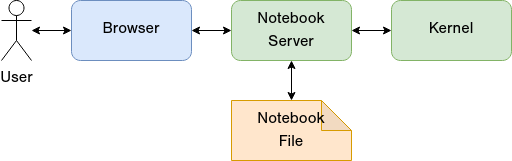
\includegraphics[width=0.8\textwidth]{notebook-architecture.png}
	\caption{Architecture of the Jupyter notebook computing environment.}
	\label{fig:notebook_architecture}
\end{figure*}

\subsection{Notebook Architecture}

Many different kinds of computational notebooks exist today for many different programming languages, but all of these various implementations share a set of common features. As the Jupyter notebook has become the most prominent, we will focus our discussion on it as an illustrative example.

The architecture of a Jupyter notebook comprises four components: a web browser, a notebook server, a notebook file, and a kernel \citep{kluyver_jupyter_2016}. As illustrated in Figure \ref{fig:notebook_architecture}, the user relies on a web browser to interact with the notebook server, which reads the notebook file and renders it in the browser as a web page. This site includes individual cells, coherent bits of either code or text, in which the user can type interactively. A code cell can also be executed, an action through which the browser sends the code in the cell to the server, which routes it to the kernel, a back-end interpreter which runs the code and returns the result to the browser via the notebook server. The browser renders this result inline in the notebook beneath the code cell. Thus, computational output such as individual calculations, tables, or figures appear beside the code that generated it.

Notebook kernels are language-specific. Hundreds of Jupyter kernels exist for dozens of different programming languages. The most popular languages for data science are all supported, including Python, R, and Julia.

\begin{figure*}[tbp]
	\centering
	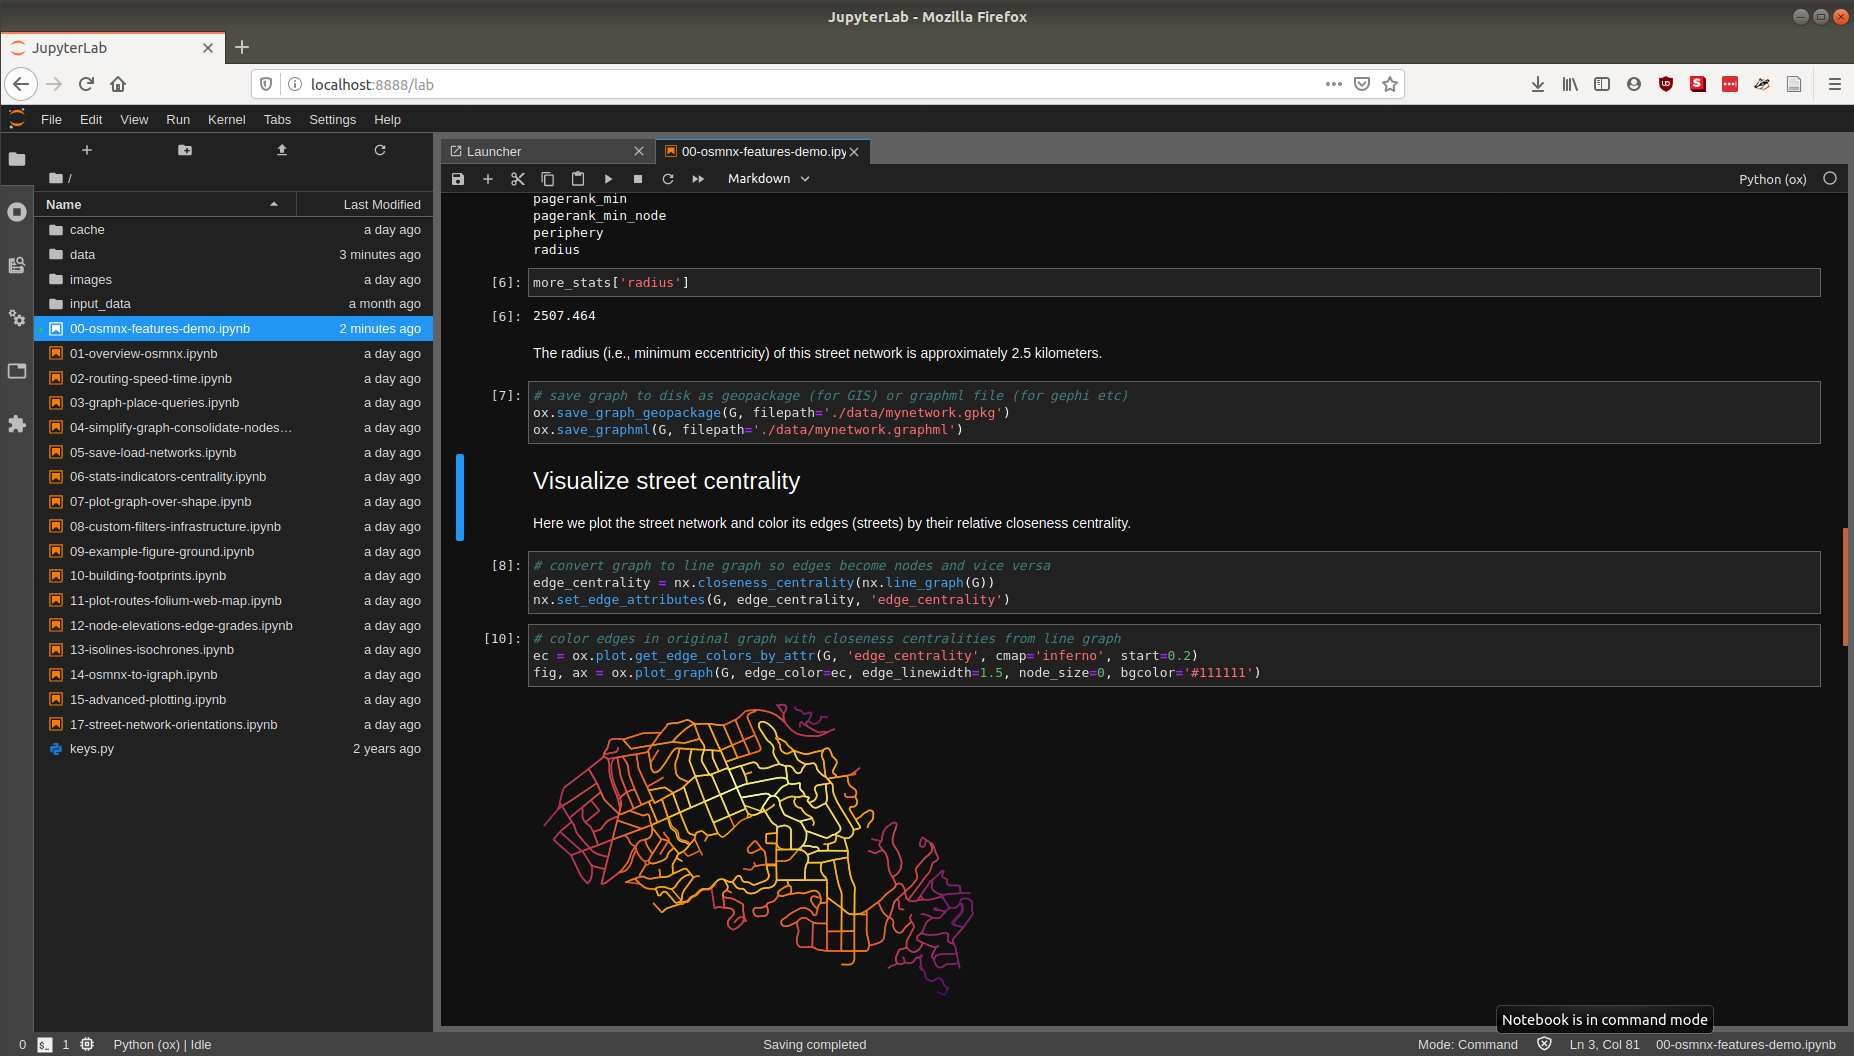
\includegraphics[width=1\textwidth]{jupyterlab-interface.png}
	\caption{The JupyterLab notebook interface.}
	\label{fig:jupyterlab_interface}
\end{figure*}

\subsection{Notebook Usage}

As discussed briefly above, a web browser renders the user interface of the computational notebook. In the Jupyter ecosystem, this user interface is called JupyterLab. JupyterLab shares many common user interface elements with other computational notebooks. It primarily consists of a main work area and a sidebar to browse files and running kernels, as illustrated in Figure \ref{fig:jupyterlab_interface}. 

The main work area contains the currently open notebooks. Here, notebooks can be created, edited, and executed. Users can add or remove notebook cells, move cells around to reorder their execution, type code or markdown text into cells, or run one or more cells. Given the interactive paradigm, a cell or cells can be run once or many times repeatedly, and cells may be run in any order the user desires. Due to this possibly nonlinear flow of execution, it is important to periodically restart the kernel and run all cells to ensure that objects are defined and used in the expected order of operations.

Computational notebooks are increasingly used today in pedagogy, research, and practice. Instructors use them to introduce students to coding and data science because they can show the results of each computation, step by step, and explain each new language detail along the way \citep{reades_teaching_2020}. Researchers use them to document, explain, and visualize their research questions, hypotheses, data, experiments, and results inline with the code \citep{perkel_why_2018}. Software developers use them to provide visual, narrative usage examples and demonstrations of their software packages for newcomers to learn how they work \citep{boeing_urban_2020}. All of a computational notebook's code, text, and multimedia content is stored in a single notebook file, so they can easily be shared and distributed and they work well in collaborative version control systems. Because the specification used to store notebooks is open and text-based, a wide ecosystem of tools exist to convert to and from the notebook file format into other formats used in scientific work (e.g., PDF, markdown, Microsoft Word).

\section{Open-Notebook GIS}

Computational notebooks are not specific to GIS. However, the nature of GIS work makes notebooks an essential building block for modern geospatial workflows. Although their domain of use is much wider and spans almost every branch of (interactive) scientific computing, several of their features fit particularly well with existing well-documented needs in the GIS discipline. In fact, if computational notebooks did not exist, the GIS community would have to invent them. Their growing necessity derives from three core aspects of modern GIS that notebooks address natively: 1) the distributed nature of modern GIS software, 2) the increasingly messy nature of data, and 3) emerging trends in Open Science.

\subsection{Software Ecosystem}

The GIS software ecosystem has dramatically changed in the last decade \citep{arribas-bel_geography_2018}. Until the early 2000s, the desktop had remained the standard platform \citep{gahegan_our_2018}. A desktop-centric paradigm favored all-encompassing software covering as much functionality as possible and exposed it in a simple manner for non-technical audiences. Several subdomains in the GIS industry still operate in this paradigm (e.g. local government, military). However, most of the research community that uses (and expands) the GIS domain, as well as a nascent industry community around geographic data science, have transitioned to a different model. This new framework is characterised by a distributed and decentralised approach to software production and use, centered around coding and open source packages. In this modern context, notebooks provide an ideal tool to transparently tie together the ecosystem. Computational notebooks are built around coding rather than point-and-click desktop applications and provide explicit mechanisms to detail the \enquote{whats,} \enquote{whys,} and \enquote{hows} of the software used.

\subsection{Data Ecosystem}

Since the early 2000s, the geospatial data ecosystem has also been radically redefined. Traditional data sources available to GIS researchers (e.g., decadal censuses, official surveys, limited remote sensing) have been augmented by entirely new kinds of data from sensors such as smartphones, video camera feeds, and drones/nano-satellites. These data are not just \enquote{more} or \enquote{bigger}; they fundamentally differ from traditional data \citep{kitchin_what_2016}. Furthermore, unlike many traditional sources, they were not designed for research: transforming them requires particular effort and attention to render them usable for appropriate analytics \citep{harris_more_2017,singleton_geographic_2019}. In this context, notebooks integrate the tools required for these transformations and enable clear documentation of all the steps and decisions made by researchers in the process of turning original inputs into analysis-ready data.

\subsection{Open Spatial Science}

Finally, the GIS world has recently been a part of broader discussions concerning Open Science and reproducible research \citep{brunsdon_quantitative_2016,kedron_reproducibility_2019}. Recent scandals regarding the lack of scientific transparency and reproducibility of published results have generated attention across the scientific world. In turn, much of the response has coalesced around the notion of open science, which focuses on ensuring that scientific research is adequately documented and disseminated so third parties can fully understand and replicate the workflow \citep{koster_fueling_2020,poorthuis_being_2019,rey_show_2009}. In GIS, reproducibility also entails the underlying technology supporting the research. Although early GIS work was mostly mathematical---and thus easily fully documented in journal articles---the evolution of desktop GIS made it difficult to maintain a close correspondence between the numerous operations carried out on the researcher's computer and the final results presented in an article. Computational notebooks present an alternative where transparency and reproducibility are built-in, nudging researchers toward Open Science.

In sum, \enquote{open-notebook GIS} ties together modern geospatial software and data ecosystems for open science. Notebooks help integrate the modern geospatial software landscape although they are not geospatial software themselves. They help leverage new forms of data whose availability and accessibility relies on modern technologies, such as application programming interfaces (APIs) or distributed databases. And they encourage analytical transparency, documentation, and reproducibility.

\section{Notebooks Are Not Enough}

As important as computational notebooks are becoming to modern GIS, they alone are necessary but insufficient. Notebooks can rather be seen as the \enquote{glue} that ties together the various distributed components that make up the modern geospatial scientific stack. This broader landscape of modern GIS---of which computational notebooks are a core component---has two more key building blocks: open source packages and transferable platforms.

Open source packages are the main vehicle through which scientific software in general, but GIS in particular, is currently distributed (\hl{REF}). Packages are compilations of code that allow users to reuse and reapply their functionality in a variety of contexts. Open source refers to the license and set of rights that are granted to the user, which typically include examining, modifying, and redistributing the code that makes up the package. Open source packages offer more modular and flexible ways of distributing software than legacy desktop GIS---albeit with an expectation that the user is comfortable writing at least some computer code. The open source model has proven more efficient and agile at incorporating new technology and supporting a wider variety of use cases. In this model, computational notebooks integrate different packages and provide a natural interface that replaces the graphical user interface (GUI) of legacy desktop GIS.

By \enquote{transferable platforms} we refer to the broader lower-level set of software and infrastructure required to execute (GIS) software in a way that is easy to transfer across hardware and users. Modern scientific software stacks are complex and delicate. They rely on many interconnected components that must be installed in a specific way (i.e., version, compiler, etc.) to maintain compatibility with every other piece of the whole. Building and replicating these environments is non-trivial and can hinder reproducibility.

The motivation behind transferable platforms is to develop tools and practices that make it easier to distribute these complex stacks in reliable ways. No single standard method of adopting transferable platforms currently exists, but a set of connected components are emerging around package managers like \texttt{conda} and containerization technologies like Docker. In this context, computational notebooks provide the main user interface to a pre-built, fully compartmentalized platform. Their adoption thus makes it easier to distribute transferable platforms in more accessible and user-friendly ways.

\begin{figure*}[!tb]
	\centering
	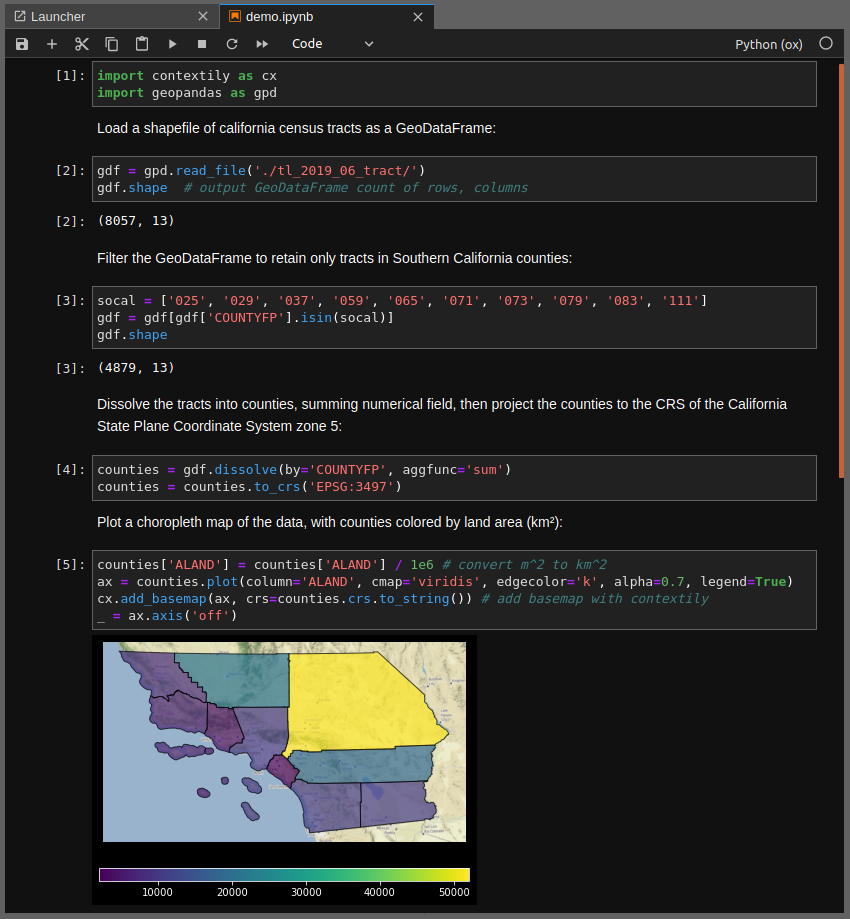
\includegraphics[width=0.9\textwidth]{code-demo.png}
	\caption{Simple real-world usage example that demonstrates basic GIS in a computational notebook, using JupyterLab and Python.}
	\label{fig:code_demo}
\end{figure*}

\section{Notebooks in Action}

Today, the geographic data science ecosystem is most robust in R (particularly the r-spatial community) and Python, where many packages exist to support spatial analysis and modeling such as \texttt{geopandas} (geospatial data wrangling), \texttt{PySAL} (advanced spatial analytics and modeling), \texttt{matplotlib} (data visualization), \texttt{OSMnx}  (street network modeling and analytics), \texttt{folium} (web mapping), and many more (see the Additional Resources section for links). These tools allow data scientists to fully replace legacy desktop GIS software with reproducible, universal analytics workflows in computational notebooks.

We conclude this chapter with a real-world usage example using JupyterLab and Python that presents a set of GIS standard operations in a computational notebook, illustrated in Figure \ref{fig:code_demo}. In cell 1, we import the \texttt{contextily} package for retrieving basemap tiles and give it the shorter \texttt{cx} handle, then we import the \texttt{geopandas} package for geospatial data handling and give it the shorter \texttt{gpd} handle. In cell 2, we use \texttt{geopandas} to read an ESRI shapefile containing all the census tracts in California, turn it into a GeoDataFrame, and output the shape of the resulting GeoDataFrame. We have 8,057 rows (i.e., census tracts) and 13 columns (i.e., variables).

In cell 3, we create a list of all the county IDs in Southern California, then filter the GeoDataFrame to only retain tracts whose county IDs appear in that list. Outputting the shape of the resulting GeoDataFrame here reveals that we have retained only 4,879 of the original 8,057 tracts. In cell 4, we dissolve and project the GeoDataFrame. First we aggregate the tracts up to the county level with a standard spatial dissolve operation and sum their numerical attributes to get new county totals. Then we project the GeoDataFrame from its original coordinate reference system (as defined in the shapefile) to a new one representing the meter-based California State Plane Coordinate System zone 5.

Finally, in cell 5, we convert the land area column from m\textsuperscript{2} to km\textsuperscript{2}, then plot a (very basic) choropleth map of the spatial data, with counties colored by land area. Then we add a basemap via \texttt{contextily}. This notebook can be executed linearly like a script by running it from the top-down, or it can be executed nonlinearly by a user choosing individual cells to run one or multiple times in an arbitrary order.

\setlength{\bibsep}{0.00cm plus 0.05cm}
\bibliographystyle{apalike}
\bibliography{GIS-BoK}

\section*{Learning Objectives}

\begin{itemize}
    \item Define computational notebooks in general without reference to individual technology platforms.
    \item Explain the difference between the notebook paradigm and traditional computer programs for GIS.
    \item Explain how to use the JupyterLab user interface.
    \item Describe the usefulness of computational notebooks in modern GIS analytics.
    \item Express the importance of computational notebooks in open (geospatial) science.
\end{itemize}

\section*{Instructional Assessment Questions}

\begin{itemize}
    \item What is the difference between JupyterLab and a computational notebook?
    \item What are the different components of a Jupyter notebook environment and how do they interrelate?
    \item How do computational notebooks help instructors teach coding?
    \item What are the advantages of using notebooks for geospatial analytics rather than legacy desktop GIS software?
    \item How do notebooks help researchers make their workflows and findings more transparent and reproducible?
\end{itemize}

\section*{Additional Resources}

\begin{itemize}
    \item \href{https://jupyter.org/}{Project Jupyter}
    \item \href{https://geopandas.org/}{geopandas}
    \item \href{https://pysal.org/}{PySAL}
    \item \href{https://matplotlib.org/}{matplotlib}
    \item \href{https://osmnx.readthedocs.io/}{OSMnx}
    \item \href{https://scitools.org.uk/cartopy/docs/latest/}{cartopy}
    \item \href{https://python-visualization.github.io/folium/}{folium}
    \item \href{https://doi.org/10.5281/zenodo.1135210}{a course on geographic data science, using notebooks and containerization}
\end{itemize}

\section*{Associated Image}

Figure \ref{fig:jupyterlab_interface} can be used as the associated image.

\end{document}
